\chapter{Resultados e Discussões}

\section{Resultados para $ F_0 $}

Os resultados da adaptação do filtro para uma força $F_0(t) = A_0 sin(2\pi f_0 t)$ com $ N=1000 $ são mostrado na \cref{fig:F0_1000_90_conv}. O número de coeficientes do filtro ($ N_c $) e o fator de convergência ($ \mu $) utilizados são apresentados na figura.

\begin{figure}[!h]
	\centering
	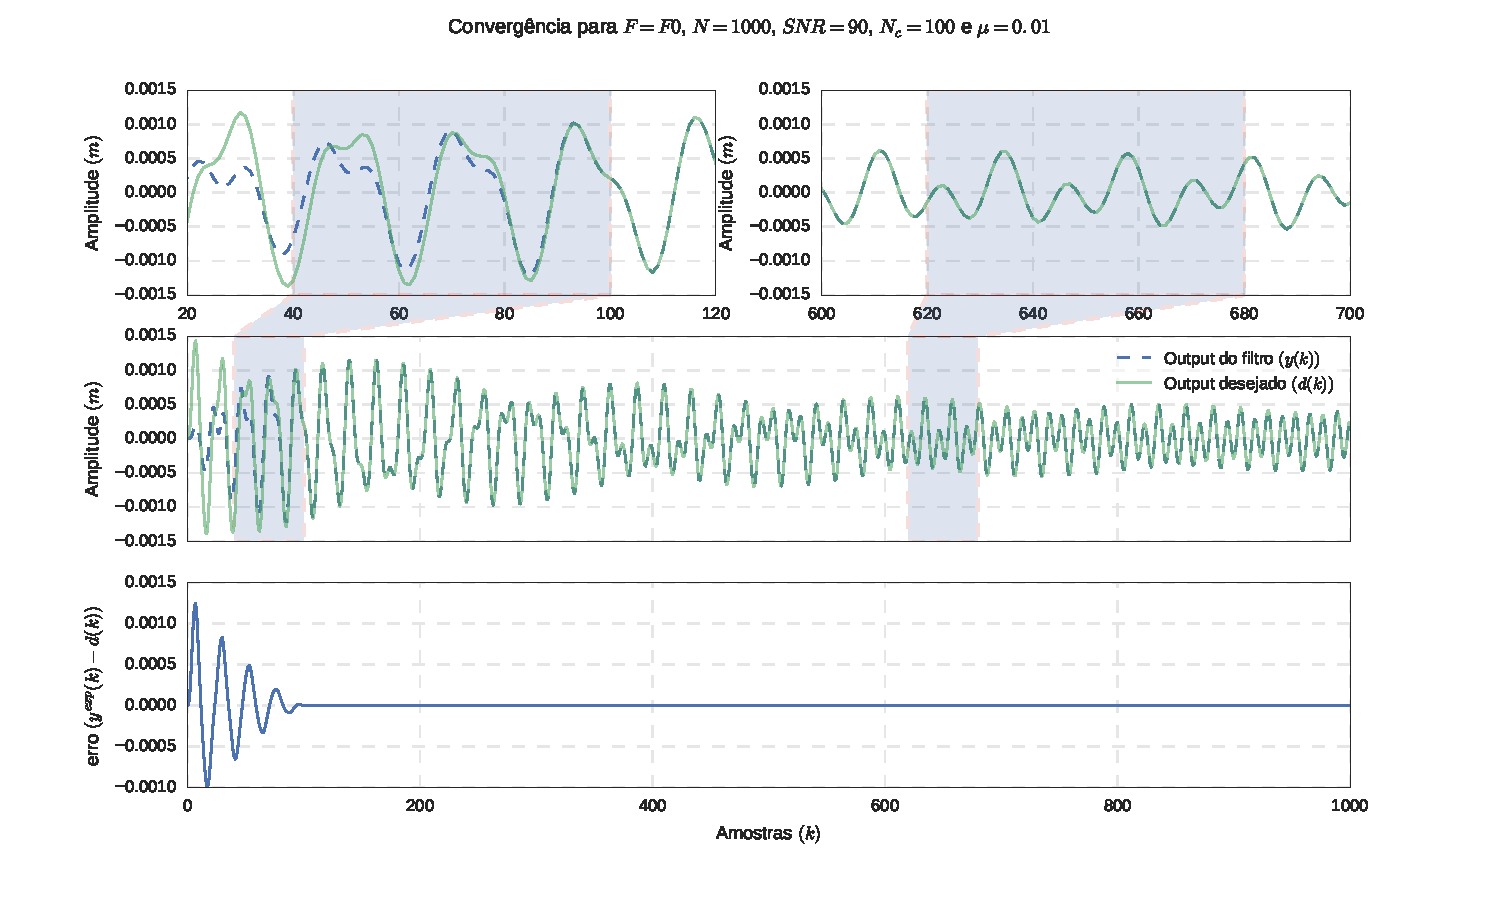
\includegraphics[scale=0.7]{IMGS/F0_1000_90_conv}
	\caption{Evolução do filtro para $ F=F_0 $ e $ N=1000 $}
	\label{fig:F0_1000_90_conv}
\end{figure}

Assim como mostrado por \citet{castello2005experimental}, no caso analisado o fenômeno de anti-ressonância também não foi capturado pelo LMS.